\providecommand{\curso}{Octavo Básico A}
\providecommand{\colegio}{Colegio Divina Pastora}
\providecommand{\tituloDocumento}{Prueba 1}
\providecommand{\subtituloDocumento}{Teorema de Pitágoras}

\documentclass{cdplf-prueba}

\begin{document}

\begin{tcbraster}[enhanced,raster columns=4,raster width=\linewidth,raster column skip=3pt,raster force size=false]
    \begin{caja}[title={\sffamily\scshape\bfseries Nombre},height=30pt,add to width=4.5cm]
    \end{caja}
    \begin{caja}[title=\faIcon{calculator},height=30pt,add to width=-2.5cm]
    \end{caja}
    \begin{caja}[title={\sffamily\scshape\bfseries Puntaje},height=30pt,add to width=-1cm]
    \end{caja}
    \begin{caja}[title={\sffamily\scshape\bfseries Nota},height=30pt,add to width=-1cm]
    \end{caja}                    
\end{tcbraster}

\subsection*{Objetivos de la evaluación}
\begin{itemize}[]
    \item Explicar, de manera concreta, pictórica y simbólica, la validez del teorema de Pitágoras y aplicar a la resolución de problemas geométricos y de la vida cotidiana, de manera manual y/o con software educativo.
    \item Explicar y fundamentar: 
    \begin{itemize}[label=\textbullet]
        \item   Soluciones propias y los procedimientos utilizados.
        \item   Resultados mediante definiciones, axiomas, propiedades y teoremas.
    \end{itemize}
 
\end{itemize}

\subsection*{Instrucciones generales}

La evaluación es individual y con nota al libro. Si usted lo decide, puede usar calculadora 
en el desarrollo de la evaluación. Quienes no usen calculadora tendrán una escala de corrección al 
40\% de dificultad, para quienes usen calculadora la escala será al 60\%.  

\subsection*{Pauta de cotejo}

En la corrección de la evaluación, se asignará puntaje a cada respuesta según
los criterios que se encuentran detallados en la tabla a continuación.

\begin{center}
    \begin{tblr}{width=\linewidth,colspec={X[1,c]|X[6]}, hline{1,Z} = {1}{-}{}, hline{1,Z} = {2}{-}{}, 
        hlines, cells={valign=m}, row{1} = {bg=black!15}}
        Puntaje asignado & \SetCell{c} Criterios o indicadores \\
        +50\% & Señala clara y correctamente cuál es la solución o el resultado de la pregunta hecha
        en el enunciado. \\ 
        +50\% & Incluye un desarrollo que relata de manera clara y ordenada los procedimientos 
         \mbox{necesarios} para solucionar la problemática. En caso de estar incompleto o con 
         \mbox{errores} el desarrollo, se asignará puntaje parcial si se muestra dominio de los 
         con\-tenidos y conceptos involucrados. \\
        0\% &  La respuesta es incorrecta. De haber desarrollo, este tiene errores conceptuales.\\
    \end{tblr}    
\end{center}

\vspace*{\fill}
\begin{center}
    \begin{tikzpicture}[ampersand replacement=\&,]
        %\node (A) [opacity=0.4] {\includegraphics[width=2cm]{../flork3.jpg}};
        \node (B) [font=\slshape,text width=12cm]
        {``Cree en ti mismo y en lo que eres. Sé consciente de que hay algo en tu interior %
        que es más grande que cualquier obstáculo''};
        \node [left=0mm of B,opacity=0.4] {\pgfornament[width=2cm]{37}};
        \node [right=0mm of B,opacity=0.4] {\pgfornament[width=2cm]{38}};
    \end{tikzpicture}
\end{center}
\vspace*{\fill}
\newpage

%\parte 
\begin{tcolorbox}[boxrule=1pt,colback=white,leftrule=3mm]
    \raggedright Resuelva los problemas que se encuentran a continuación. Para esto, no olvide 
    incluir un desarrollo pertinente y la respuesta al enunciado en los espacios señalizados.        
\end{tcolorbox}

\subsection[]{} Calcule la medida del lado faltante en cada caso [2 puntos c/u].

\begin{enumerate}[label={\bfseries\alph* -.},itemsep=1cm,leftmargin=1.5cm]
    \item \begin{tcolorbox}[blanker,sidebyside,lefthand width=.4\linewidth,height=5cm,box align=top,halign upper=center]
        \tikz[line width=1pt,every node/.style={}]{\draw (0,0) -- node [text width=1cm,draw,dashed,minimum height=25pt,above=5pt,anchor=south east] {} (20:4cm) -- node [midway,right=5pt] {12} ([turn]-90:3cm) -- node [midway,below=5pt] {15} cycle;
            \draw (20:4cm) -- ([turn]-90:10pt) -- ([turn]-90:10pt) -- ([turn]-90:10pt);}
        \tcblower
        \begin{malla}[]
        \end{malla}
    \end{tcolorbox}
    \item \begin{tcolorbox}[blanker,sidebyside,lefthand width=.4\linewidth,height=5cm,box align=top,halign upper=center]
        \tikz[line width=1pt,every node/.style={midway}]{\draw (0,0) -- node [midway,left=5pt] {12} (-80:3cm) -- node [midway,below=5pt] {16} ([turn]90:4cm) -- node[draw,rounded corners,minimum height=25pt,dashed,text width=1cm,above=5pt,anchor=south west] {} cycle;
            \draw (-80:3cm) -- ([turn]90:10pt) -- ([turn]90:10pt) -- ([turn]90:10pt) -- cycle;}
        \tcblower
        \begin{malla}[]
            
        \end{malla}
    \end{tcolorbox}
    \item \begin{tcolorbox}[blanker,sidebyside,lefthand width=.4\linewidth,height=5cm,box align=top,halign upper=center]
        \tikz[line width=1pt,every node/.style={midway}]{\draw (0,0) -- node[text width=1cm, minimum height=25pt,draw,rounded corners,dashed,anchor=north west,below right=5pt] {} (30:3cm) -- node [right=5pt] {24} ([turn]90:4cm) -- node [left=5pt] {25} cycle;
            \draw (30:3cm) --  ([turn]90:10pt) -- ([turn]90:10pt) -- ([turn]90:10pt) -- cycle;}
        \tcblower
        \begin{malla}[]
            
        \end{malla}
    \end{tcolorbox}
\end{enumerate}

%\pregunta 
\subsection{} Calcule el área [1 punto] y perimetro [3 puntos] de la figura sombreada.

\begin{center}
    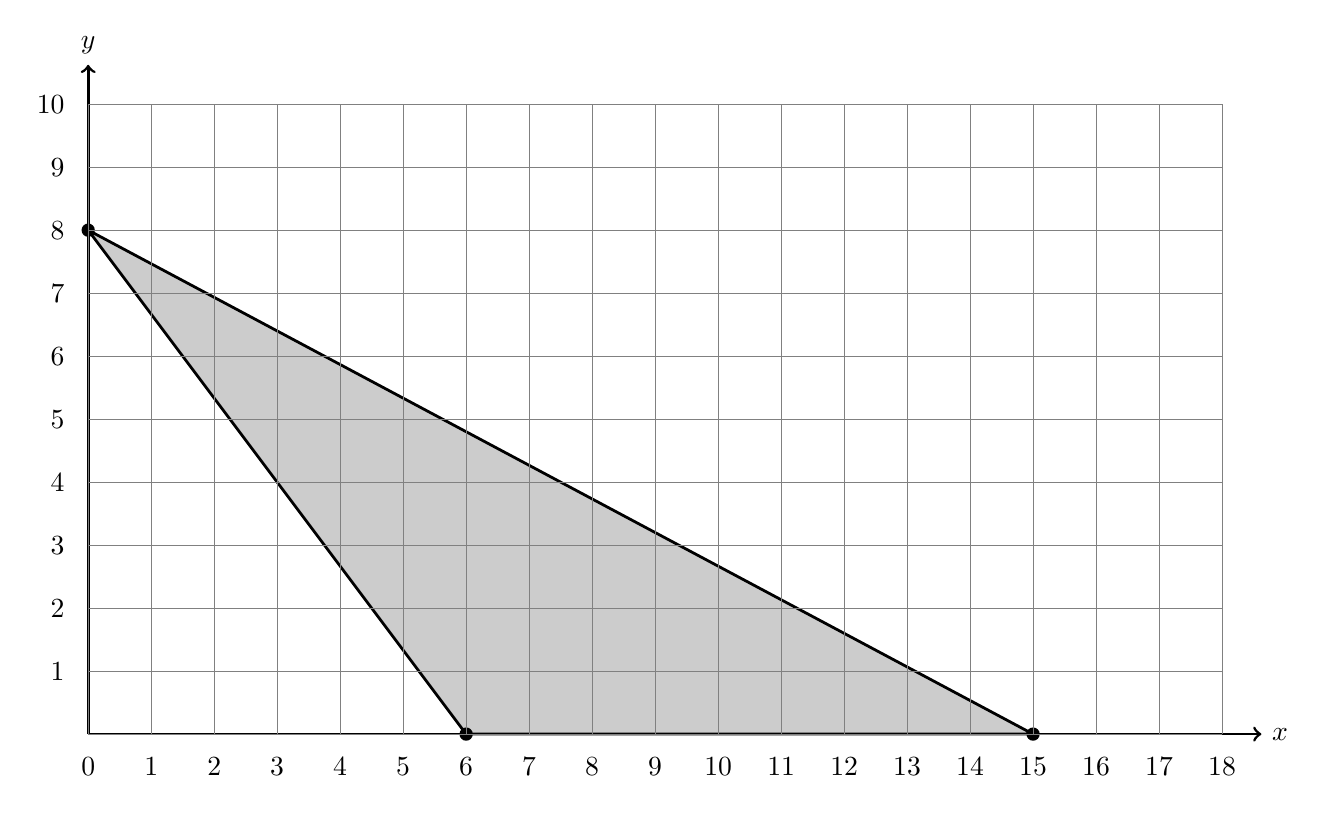
\begin{tikzpicture}[scale=0.8]
        \draw[->,shorten >=-5mm,line width=1pt] (0,0) -- (0,10) node[pos=1,above,yshift=5mm] {$y$};
        \draw[->,shorten >=-5mm,line width=1pt] (0,0) -- (18,0) node[pos=1,right,xshift=5mm] {$x$};
        \foreach \x in {0,...,18} {
            \node[below=5pt] at (\x,0) {$\x$};
        }
        \foreach \y in {1,...,10} {
            \node[left=5pt] at (0,\y) {$\y$};
        }
        \draw[line width=1pt,fill=black!20] (0,8) -- (6,0) -- (15,0) -- (0,8);
        \fill (0,8) circle (3pt);
        \fill (6,0) circle (3pt);
        \fill (15,0) circle (3pt);
        \draw[help lines] (0,0) grid (18,10);
    \end{tikzpicture}
\end{center}

\begin{tcolorbox}[enhanced,inherit height,colback=white,colframe=black,boxrule=1pt,underlay boxed title={\begin{tcbclipinterior}
    \draw[help lines,step=5mm] (interior.south west) grid (interior.north east);\end{tcbclipinterior}},title=Desarrollo,attach boxed title to top left={yshift=-\tcboxedtitleheight/2,xshift=10pt},
    boxed title style={colback=white},coltitle=black,height=9cm]
\end{tcolorbox}

\begin{tcolorbox}[enhanced,inherit height,colback=white,colframe=black,boxrule=1pt,underlay boxed title={\begin{tcbclipinterior}
    \draw[help lines,step=5mm] (interior.south west) grid[xstep=0] (interior.north east);\end{tcbclipinterior}},title=Respuesta,attach boxed title to top left={yshift=-\tcboxedtitleheight/2,xshift=10pt},
    boxed title style={colback=white},coltitle=black,height=20mm]
\end{tcolorbox}

%\desarrollo[8cm]
%\respuesta[3]

% \newsavebox\mybox
% \sbox{\mybox}{<content>}
% \wd\mybox % width
% \ht\mybox % height
% \dp\mybox % depth
%
\NewDocumentCommand{\sT}{m}{\resizebox{15pt}{!}{$\triangle_{#1}$}}%
\NewDocumentCommand{\sC}{m}{\resizebox{15pt}{!}{$\square_{#1}$}}

%\pregunta 
\subsection[]{} Determine, \textbf{sin usar el teorema de Pitágoras}, el valor 
de la hipotenusa para un triángulo rectángulo con catetos de largo 6 y 8 
[Son cuatro pasos, 1 punto c/u].

%% 9 12 15
\def\cuadradoCompleto{%
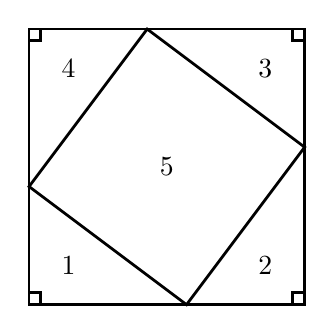
\begin{tikzpicture}[x=0.5cm,y=0.5cm]
    \pgfmathsetmacro{\a}{3};
    \pgfmathsetmacro{\b}{4};

    \draw[line width=1pt] (0,0) rectangle (\a+\b, \a+\b);
    \draw[line width=1pt] (0,\a) -- (\b,0) -- (\a + \b, \b) -- (\a,\a+\b) -- cycle;
    \draw[line width=1pt] (0,0) rectangle +(0.3,0.3);
    \draw[line width=1pt] (\a+\b,\a+\b) rectangle +(-0.3,-0.3);
    \draw[line width=1pt] (0,\a+\b) rectangle +(0.3,-0.3);
    \draw[line width=1pt] (\a+\b,0) rectangle +(-0.3,0.3);

    \node [xshift=0.5cm,yshift=0.5cm] at (0,0) {\sT{1}};
    \node [xshift=-0.5cm,yshift=0.5cm] at (\a+\b,0) {\sT{2}};
    \node [xshift=-0.5cm,yshift=-0.5cm] at (\a+\b,\a+\b) {\sT{3}};
    \node [xshift=0.5cm,yshift=-0.5cm] at (0,\a+\b) {\sT{4}};
    \node [] at (\a/2+\b/2,\a/2+\b/2) {\sC{5}};
\end{tikzpicture}}

\def\tUno{%
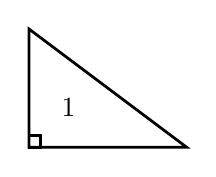
\begin{tikzpicture}[x=1cm,y=1cm,scale=0.5]
    \pgfmathsetmacro{\a}{3};
    \pgfmathsetmacro{\b}{4};
    \draw[line width=1pt] (0,0) -- (\b,0) -- (0,\a) -- cycle;
    \draw[line width=1pt] (0,0) rectangle +(0.3,0.3);
    \node [xshift=0.5cm,yshift=0.5cm] at (0,0) {\sT{1}};
\end{tikzpicture}}
\def\tDos{%
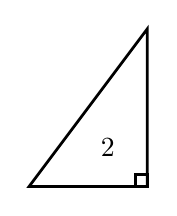
\begin{tikzpicture}[rotate=90,scale=0.5]
    \pgfmathsetmacro{\a}{3};
    \pgfmathsetmacro{\b}{4};
    \draw[line width=1pt] (0,0) -- (\b,0) -- (0,\a) -- cycle;
    \draw[line width=1pt] (0,0) rectangle +(0.3,0.3);
    \node[xshift=-0.5cm,yshift=0.5cm] at (0,0) {\sT{2}};
\end{tikzpicture}}
\def\tTres{%
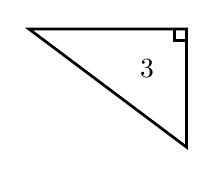
\begin{tikzpicture}[scale=0.5,rotate=180]
    \pgfmathsetmacro{\a}{3};
    \pgfmathsetmacro{\b}{4};
    \draw[line width=1pt] (0,0) -- (\b,0) -- (0,\a) -- cycle;
    \draw[line width=1pt] (0,0) rectangle +(0.3,0.3);
    \node[xshift=-0.5cm,yshift=-0.5cm] at (0,0) {\sT{3}};
\end{tikzpicture}}
\def\tCuatro{%
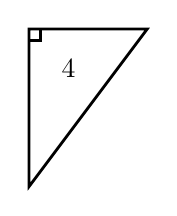
\begin{tikzpicture}[scale=0.5,rotate=270]
    \pgfmathsetmacro{\a}{3};
    \pgfmathsetmacro{\b}{4};
    \draw[line width=1pt] (0,0) -- (\b,0) -- (0,\a) -- cycle;
    \draw[line width=1pt] (0,0) rectangle +(0.3,0.3);
    \node[xshift=0.5cm,yshift=-0.5cm] at (0,0) {\sT{4}};
\end{tikzpicture}}
\def\cChico{%
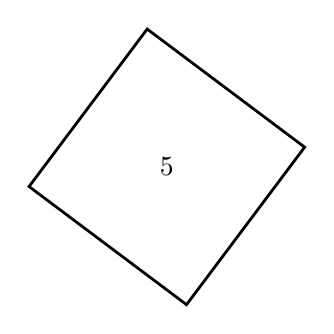
\begin{tikzpicture}[scale=0.5]
    \pgfmathsetmacro{\a}{3};
    \pgfmathsetmacro{\b}{4};
    \draw[line width=1pt] (0,\a) -- (\b,0) -- (\a + \b, \b) -- (\a,\a+\b) -- cycle;
    \node[xshift=0cm] at (\a/2+\b/2,\a/2+\b/2) {\sC{5}};
\end{tikzpicture}
}
\begin{tcolorbox}[enhanced,inherit height,colback=white,colframe=black,boxrule=1pt,title=Ayuda,attach boxed title to top left={yshift=-\tcboxedtitleheight/2,xshift=10pt},
    boxed title style={colback=white},coltitle=black]
    \begin{center}
        \begin{tikzpicture}[ampersand replacement=\&,line width=1pt,scale=0.7]
            \draw[line width=1pt,every node/.style={midway}] (0,0) -- node[left=5pt] {6} (-90:3cm) -- node [below=5pt] {8} ([turn]90:4cm) -- cycle coordinate [pos=0.5] (c);
            \draw[line width=1pt] (-90:3cm) -- ++(10pt,0) -- ++(0,10pt) -- ++(-10pt,0); 
            \node[above right=10pt of c,xshift=1cm,rounded corners,draw,dashed,inner sep=7pt] (t) {Hay que encontrar cuanto mide este lado};
            \draw[->,line width=1pt,shorten >=10pt,dashed] (t.south west) to[bend left=20] (c);
        \end{tikzpicture}
        \end{center}
    \tcblower
    y sabemos que: \textsl{``el área de la figura completa es igual a la suma del área de cada una de sus partes''}
    \resizebox{\linewidth}{!}%
    {\begin{tikzpicture}[ampersand replacement=\&]
            \node[] (A) {\cuadradoCompleto};
            \node [right=10pt of A.east,anchor=west,yshift=10pt] (B) {\Huge $=$};
            \node [right=10pt of B.east,anchor=west] (C) {
                \begin{tikzpicture}
                    \matrix[matrix of nodes,nodes in empty cells,nodes={minimum height=30pt,minimum width=10pt,anchor=center}] (m) 
                        {   \tUno \& {\Huge +} \& \tDos \& {\Huge +} \& \tTres \& {\Huge +} \&
                            \tCuatro \& {\Huge +} \& \cChico \\
                        };
                    \end{tikzpicture}
            };
    \end{tikzpicture}}
\end{tcolorbox}

\begin{tcolorbox}[enhanced,inherit height,colback=white,colframe=black,boxrule=1pt,underlay boxed title={\begin{tcbclipinterior}
    \draw[help lines,step=5mm] (interior.south west) grid (interior.north east);\end{tcbclipinterior}},title=Desarrollo,attach boxed title to top left={yshift=-\tcboxedtitleheight/2,xshift=10pt},
    boxed title style={colback=white},coltitle=black,height=9cm]
\end{tcolorbox}

\begin{tcolorbox}[enhanced,inherit height,colback=white,colframe=black,boxrule=1pt,underlay boxed title={\begin{tcbclipinterior}
    \draw[help lines,step=5mm] (interior.south west) grid[xstep=0] (interior.north east);\end{tcbclipinterior}},title=Respuesta,attach boxed title to top left={yshift=-\tcboxedtitleheight/2,xshift=10pt},
    boxed title style={colback=white},coltitle=black,height=35mm]
\end{tcolorbox}

%\includegraphics{example-image-a}
%righthand width=3cm
%\begin{tcolorbox}[blankest,sidebyside,righthand width=.3\linewidth] This is another \textbf{tcolorbox}.
%    \tcblower
%    Here, you see the lower part of the box.
%\end{tcolorbox

\end{document}